\subsection{Cài đặt các core component tiêu biểu}
\label{subsec:core-component-implementation}

Phần này tóm tắt các flow quan trọng nhất của hệ thống: điều phối AI Service, ôn tập flashcard theo SM-2, cộng tác realtime trên ghi chú, notification pipeline, đồng bộ Google Calendar và thanh toán PayOS. Các flow này được chọn vì thể hiện rõ cách backend phối hợp giữa domain service, persistence, scheduler, realtime channel và dịch vụ ngoài.

\subsubsection{Điều phối AI Service cho học liệu thông minh}
\label{subsubsec:ai-service-orchestration}

AI Service được tách khỏi backend chính để cô lập phần sinh nội dung và phân tích ngôn ngữ. Backend nhận yêu cầu tạo flashcard, exam, giải thích note, phân tích kiến thức hoặc sinh roadmap; sau đó kiểm tra quyền, chuẩn hóa dữ liệu đầu vào, gọi AI Service qua adapter và chỉ lưu kết quả sau khi đã kiểm tra định dạng. Nhờ vậy, client không gọi trực tiếp AI Service và các học liệu được sinh ra vẫn nằm trong workflow quản lý học liệu của backend.

\begin{figure}[htbp]
    \centering
    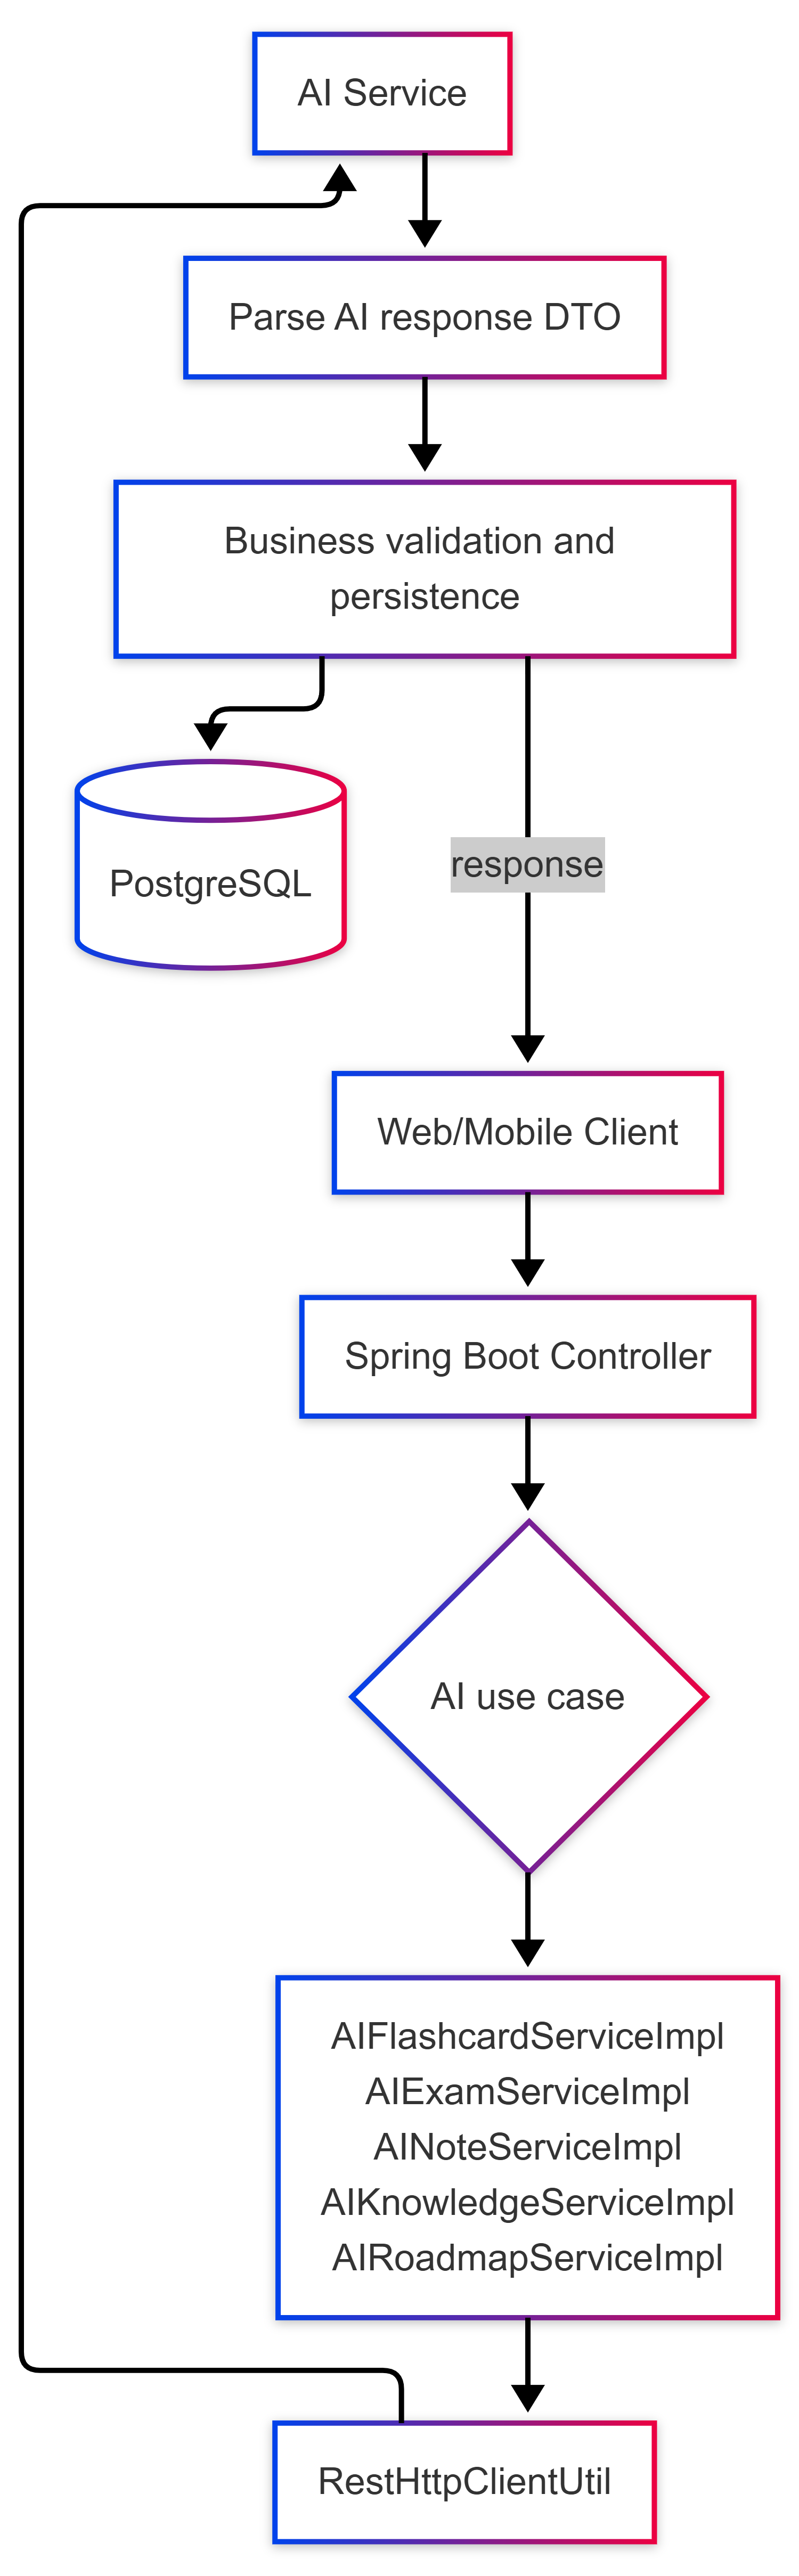
\includegraphics[width=1.5\textwidth,height=0.95\textheight,keepaspectratio]{images/chapter3/ProLearning_Arch-Detail_AI_Flow.drawio.png}
    \caption{Luồng điều phối AI Service}
    \label{fig:prolearning-architecture-detail_ai_flow}
\end{figure}

\subsubsection{Thuật toán SM-2 cho flashcard review}
\label{subsubsec:sm2-flashcard-review}

Flashcard review được cài đặt dựa trên biến thể SM-2 để lên lịch ôn tập cá nhân~\cite{supermemo_sm2}. Mỗi thẻ lưu trạng thái như \texttt{nextReviewAt}, \texttt{intervalDays}, \texttt{easeFactor} và \texttt{repetitions}; backend dùng các trường này để lấy thẻ đến hạn, ưu tiên thẻ có chu kỳ ngắn và bổ sung thẻ mới khi cần. Sau mỗi lượt học, service cập nhật lại lịch ôn, độ dễ và trạng thái nắm/không nắm thẻ để phục vụ các phiên review tiếp theo.

\begin{figure}[htbp]
    \centering
    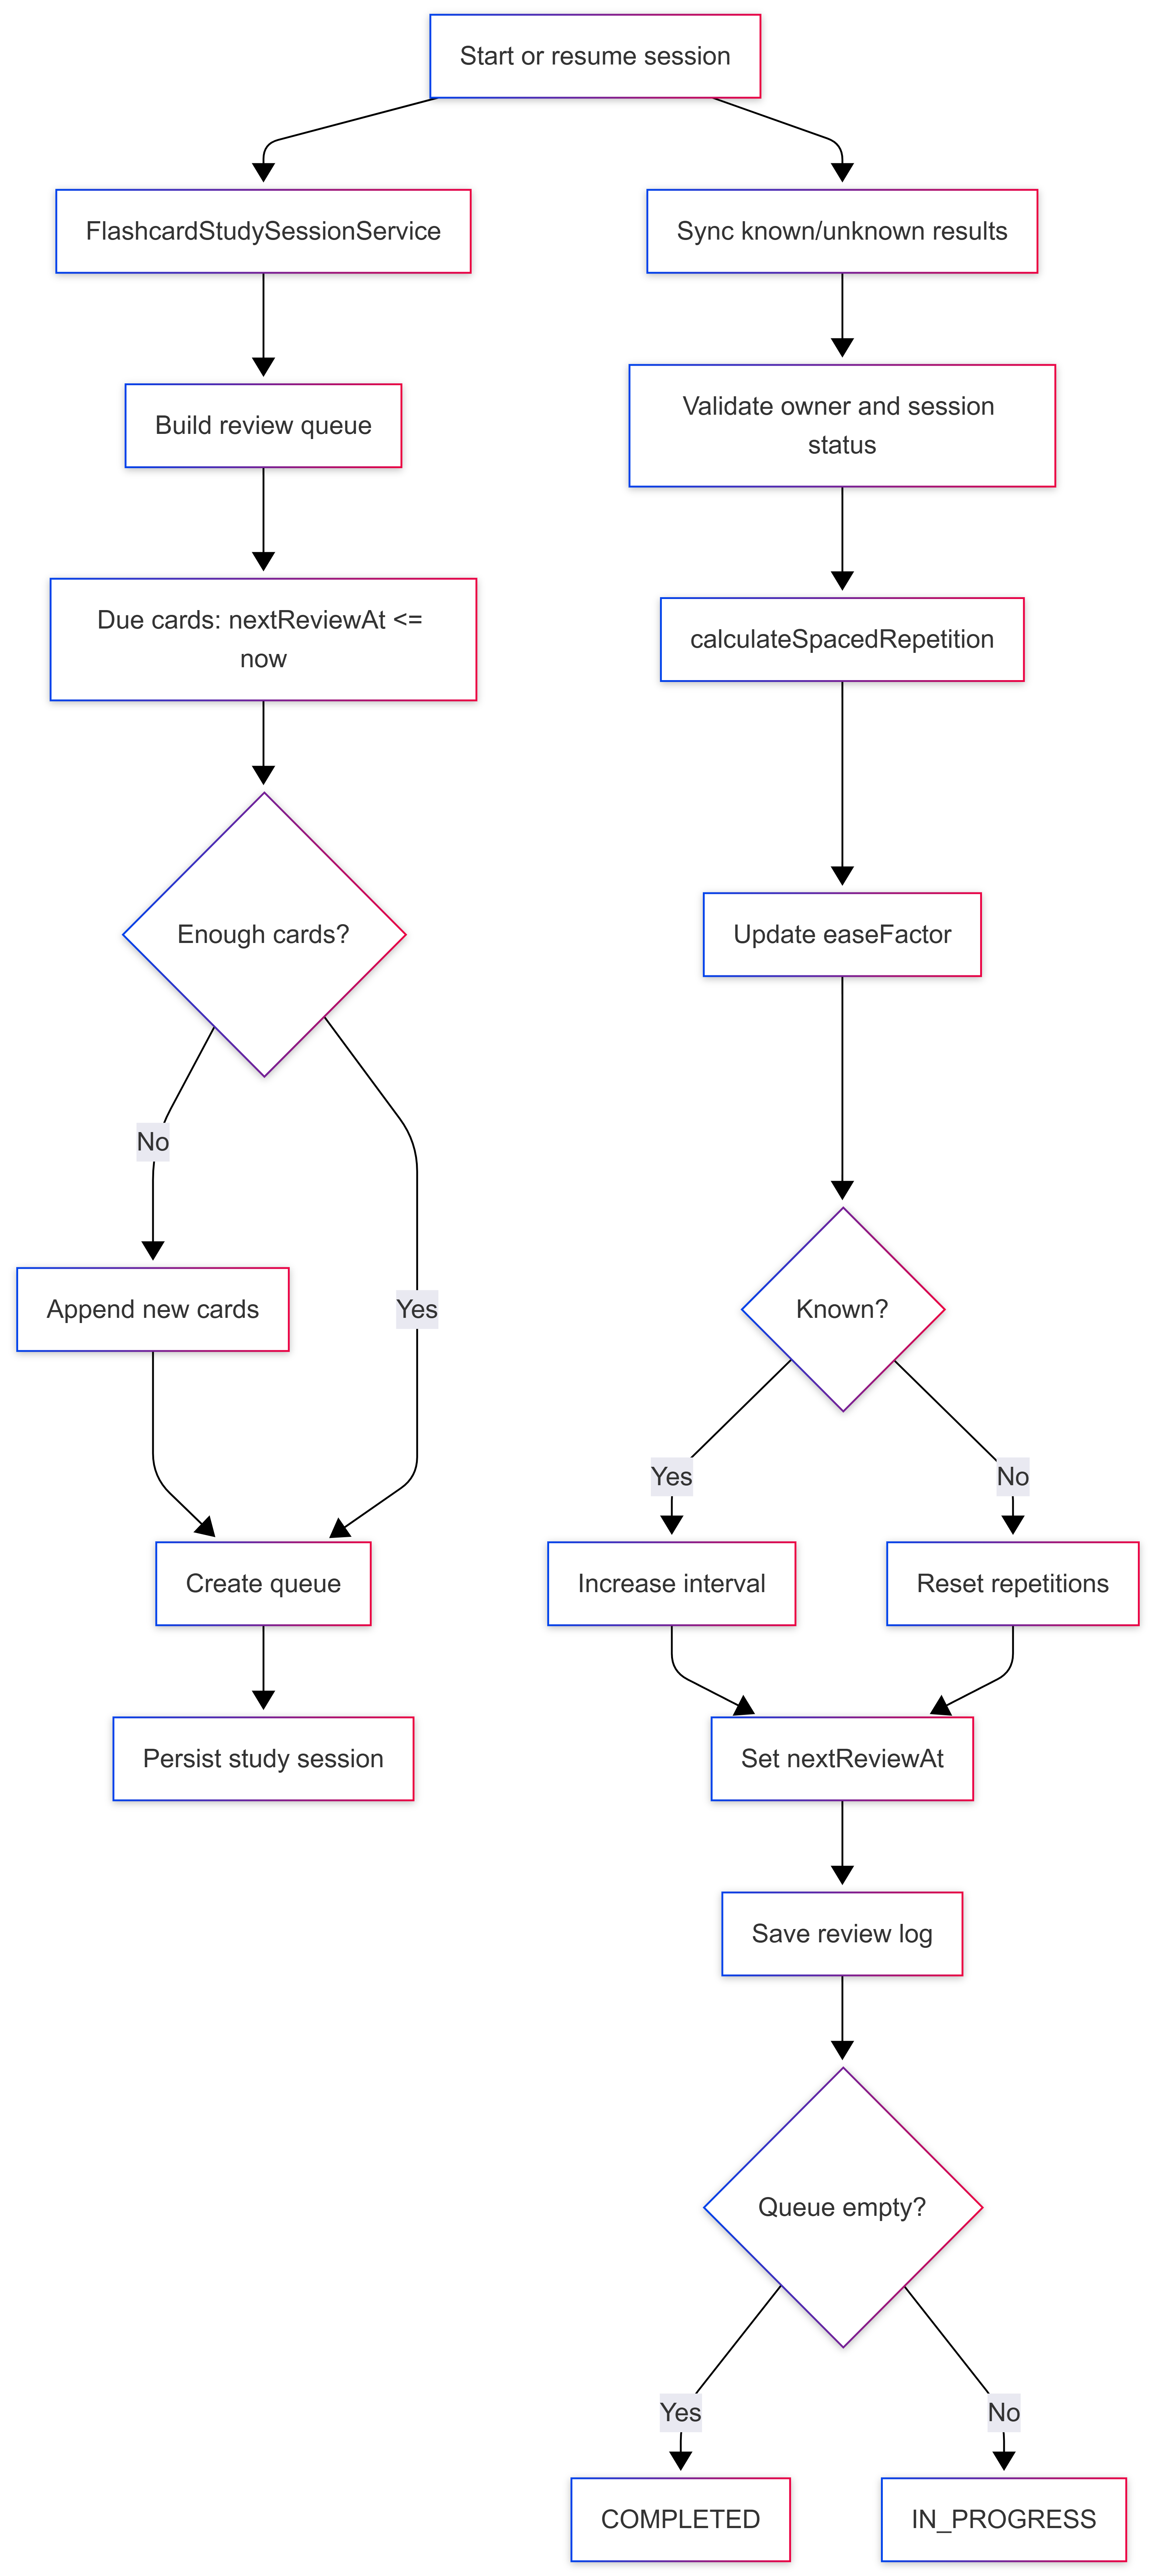
\includegraphics[width=1.5\textwidth,height=0.95\textheight,keepaspectratio]{images/chapter3/ProLearning_Arch-Detail_SM2.drawio.png}
    \caption{Luồng học và ôn tập flashcard theo SM-2}
    \label{fig:prolearning-architecture-detail_sm2}
\end{figure}

\subsubsection{Cộng tác thời gian thực trên ghi chú}
\label{subsubsec:realtime-collaboration}

Cộng tác ghi chú sử dụng WebSocket/STOMP để truyền sự kiện theo topic và Yjs để hợp nhất chỉnh sửa đồng thời~\cite{springwebsocketstomp}. Backend kiểm tra quyền tham gia note, quản lý kênh realtime, nhận snapshot cần lưu bền vững và lưu lại trạng thái có thể khôi phục trong PostgreSQL. Presence và cursor chỉ giữ ngắn hạn để giảm tải ghi database, còn nội dung chính của note được lưu theo snapshot.

\begin{figure}[htbp]
    \centering
    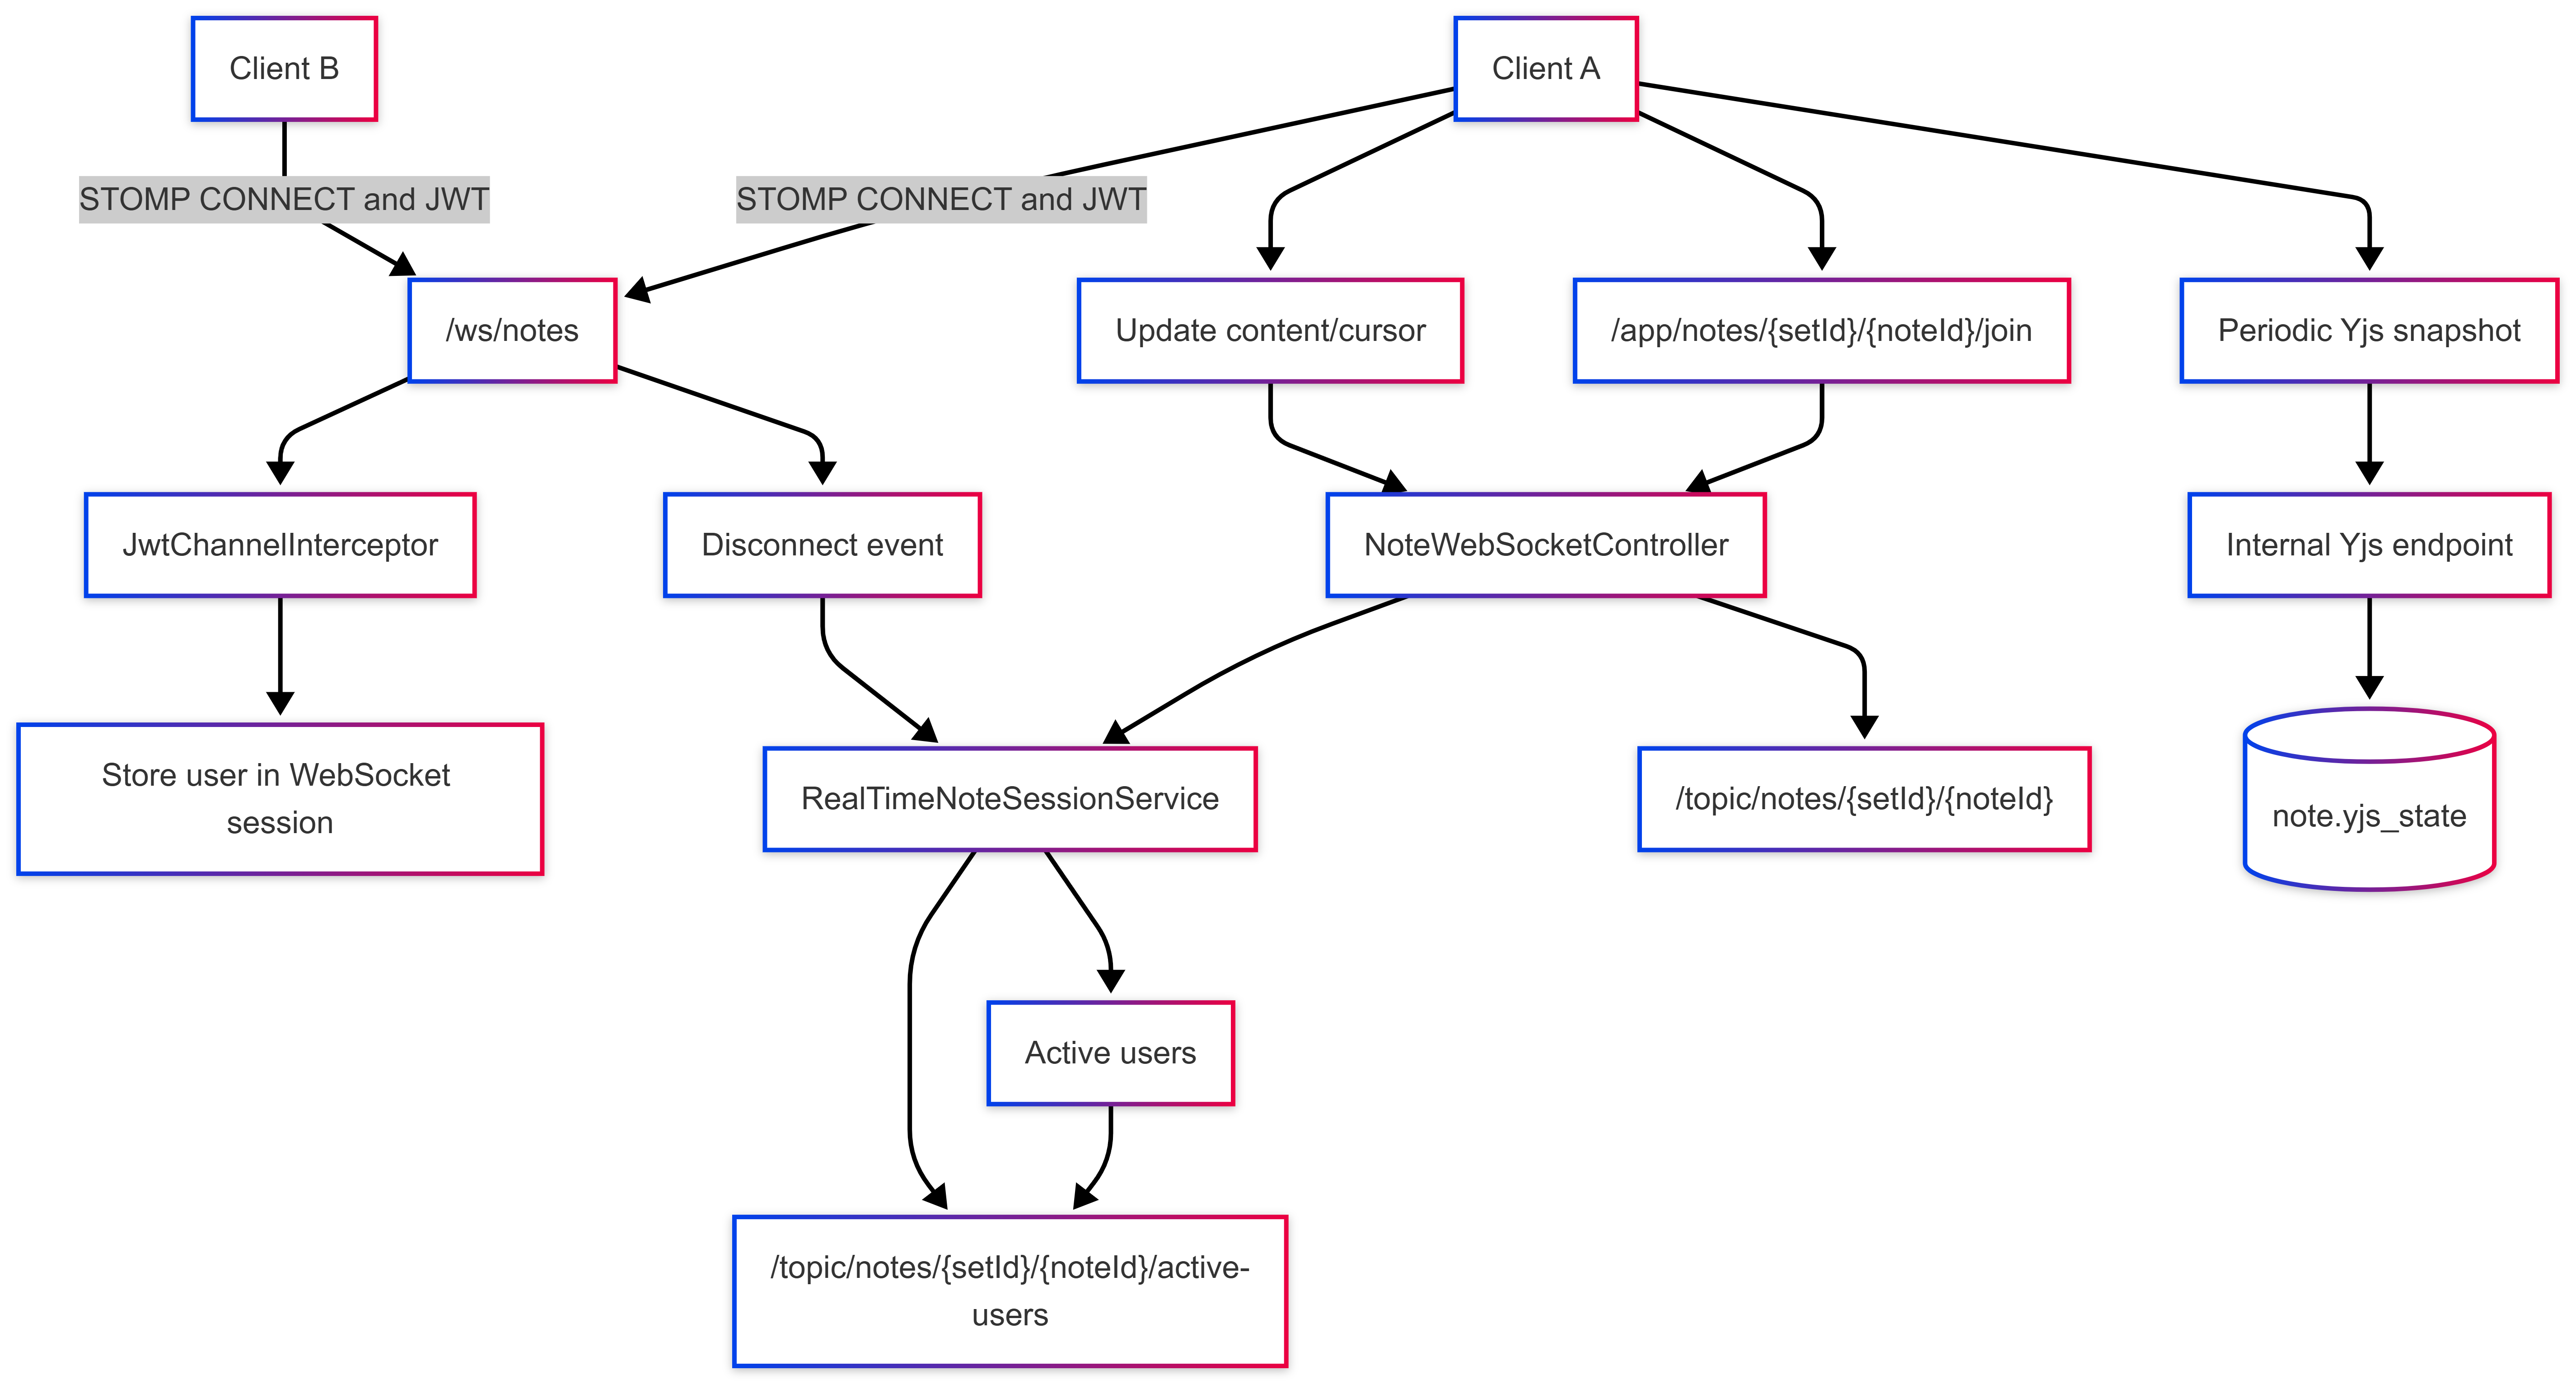
\includegraphics[width=1\textwidth,height=0.8\textheight,keepaspectratio]{images/chapter3/ProLearning_Arch-Detail_Realtime_Collab.drawio.png}
    \caption{Luồng cộng tác thời gian thực trên ghi chú}
    \label{fig:prolearning-architecture-detail_realtime_collab}
\end{figure}

\subsubsection{Pipeline thông báo đa nguồn và gửi push bất đồng bộ}
\label{subsubsec:notification-pipeline}

Notification pipeline nhận sự kiện từ nhiều nguồn như flashcard đến hạn, todo/goal sắp hết hạn, weekly summary hoặc thay đổi subscription. Backend chuẩn hóa thông báo, lưu inbox vào PostgreSQL và gửi push qua Firebase Cloud Messaging khi người dùng có thiết bị đã đăng ký~\cite{firebasefcm}. Các bước gửi push/email có thể chạy bất đồng bộ để không làm chậm request chính.

\begin{figure}[htbp]
    \centering
    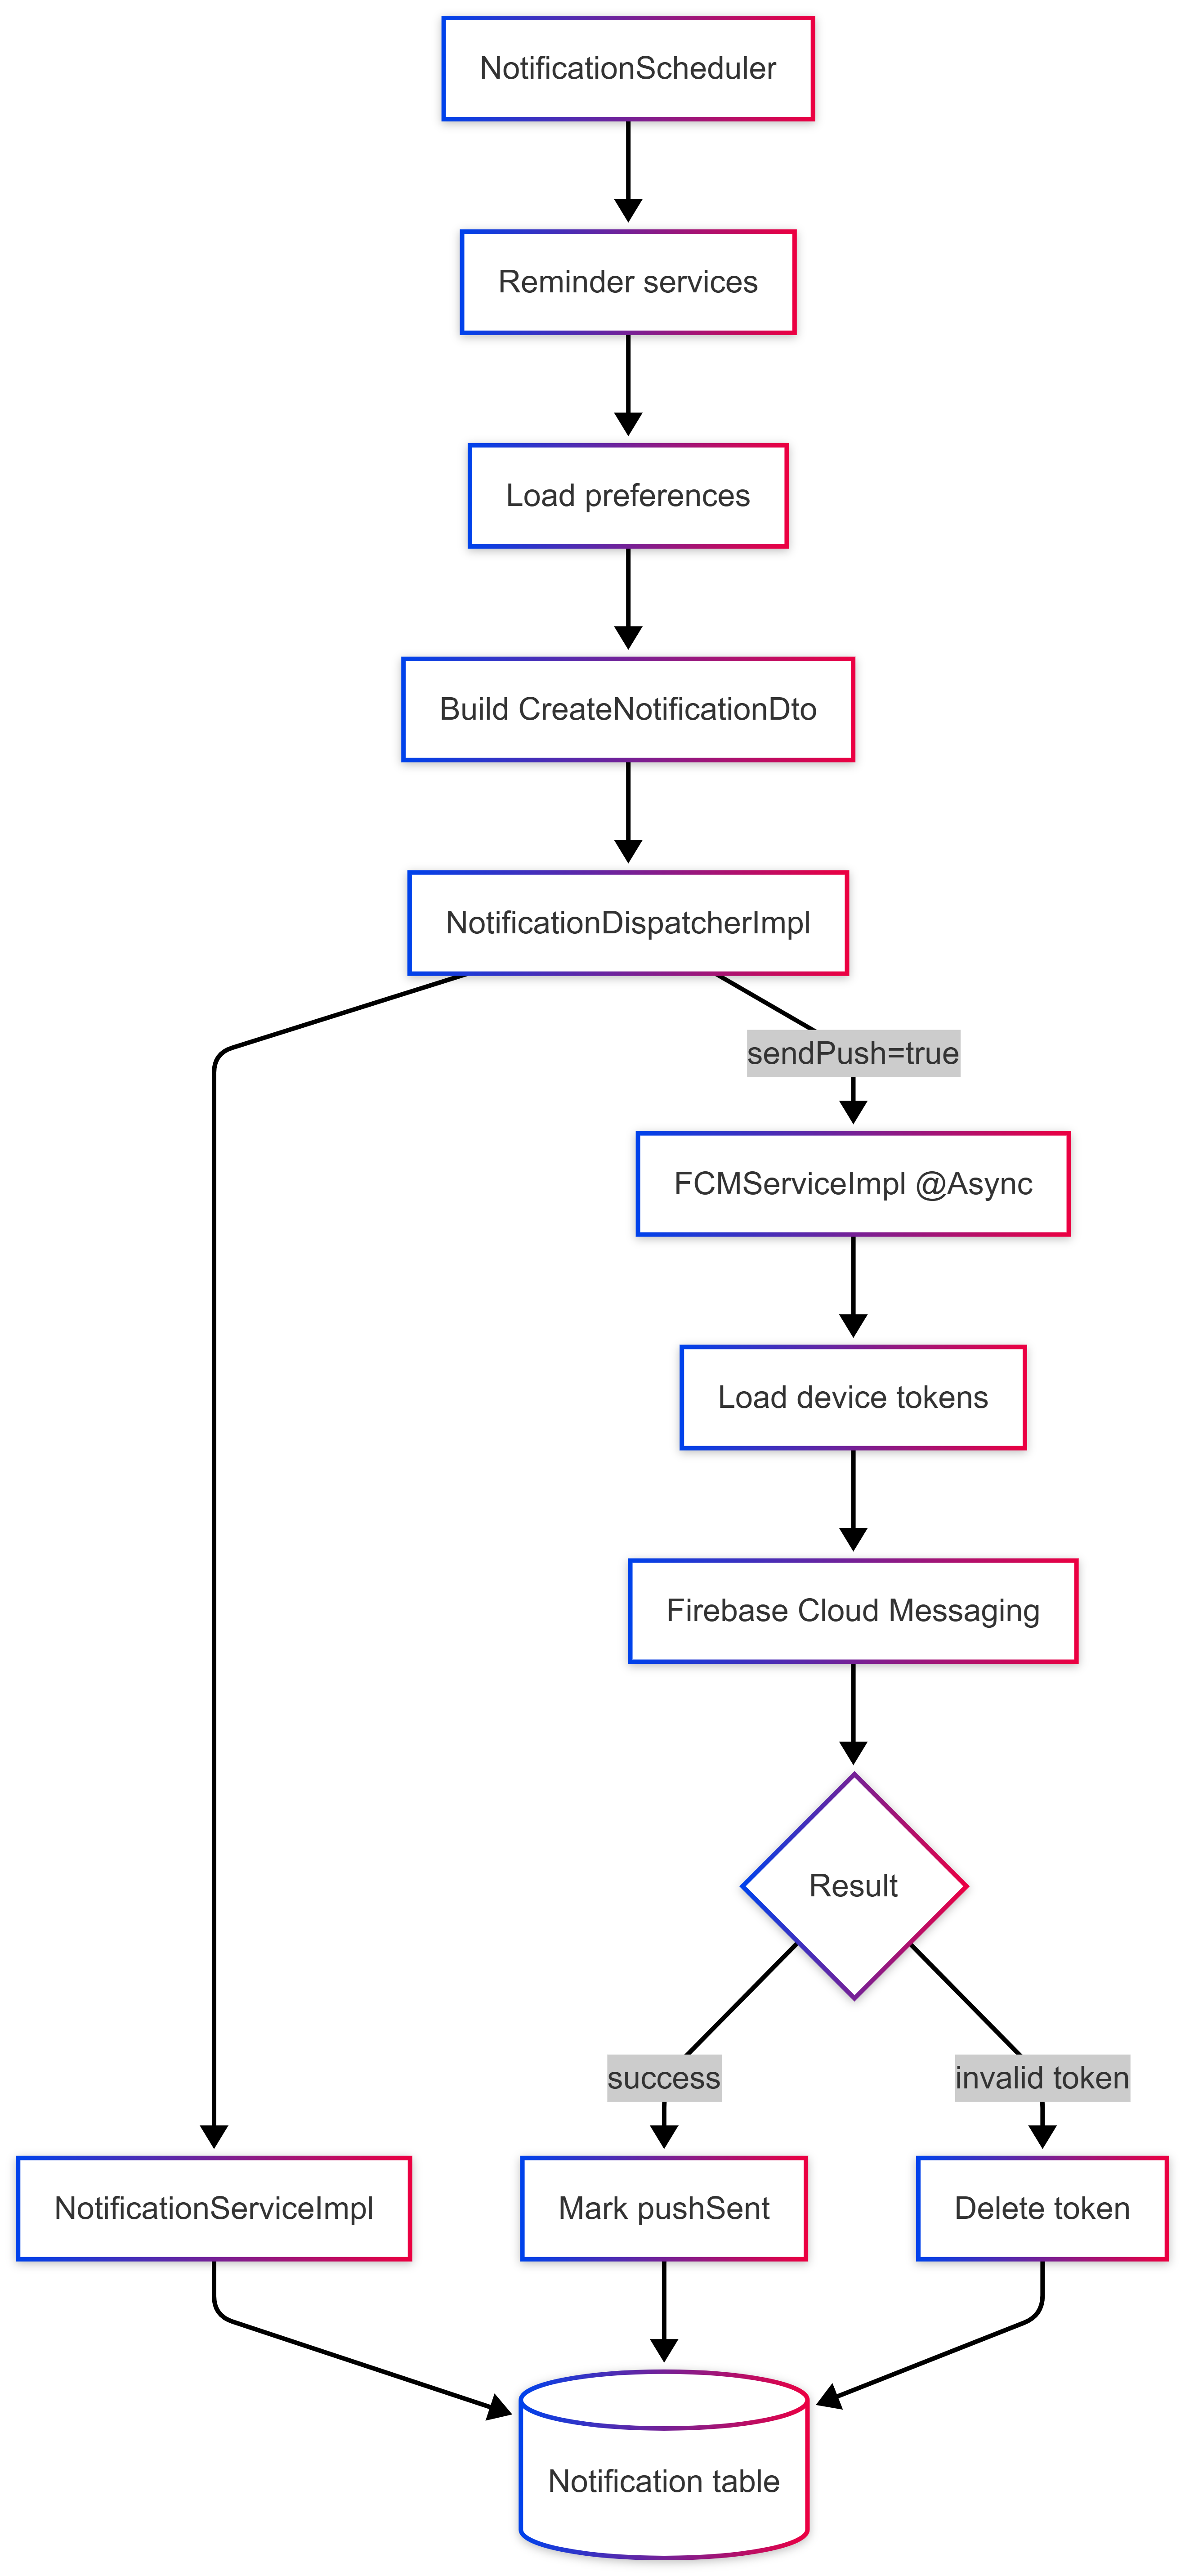
\includegraphics[width=1\textwidth,height=0.95\textheight,keepaspectratio]{images/chapter3/ProLearning_Arch-Detail_Noti_Pipeline.drawio.png}
    \caption{Luồng xử lý notification pipeline}
    \label{fig:prolearning-architecture-detail_noti_pipeline}
\end{figure}

\subsubsection{Đồng bộ Todo với Google Calendar}
\label{subsubsec:google-calendar-sync}

Đồng bộ Google Calendar được triển khai thông qua service tích hợp riêng. Backend tạo OAuth authorization URL, lưu \texttt{state} ngắn hạn trong Redis, nhận callback để lưu credential hợp lệ và dùng Google Calendar API để tạo, cập nhật hoặc xóa event tương ứng với todo có ngày đến hạn~\cite{redisoverview,googlecalendarjava}. Trạng thái đồng bộ và mã event được lưu lại để backend có thể đối soát khi todo thay đổi.

\begin{figure}[htbp]
    \centering
    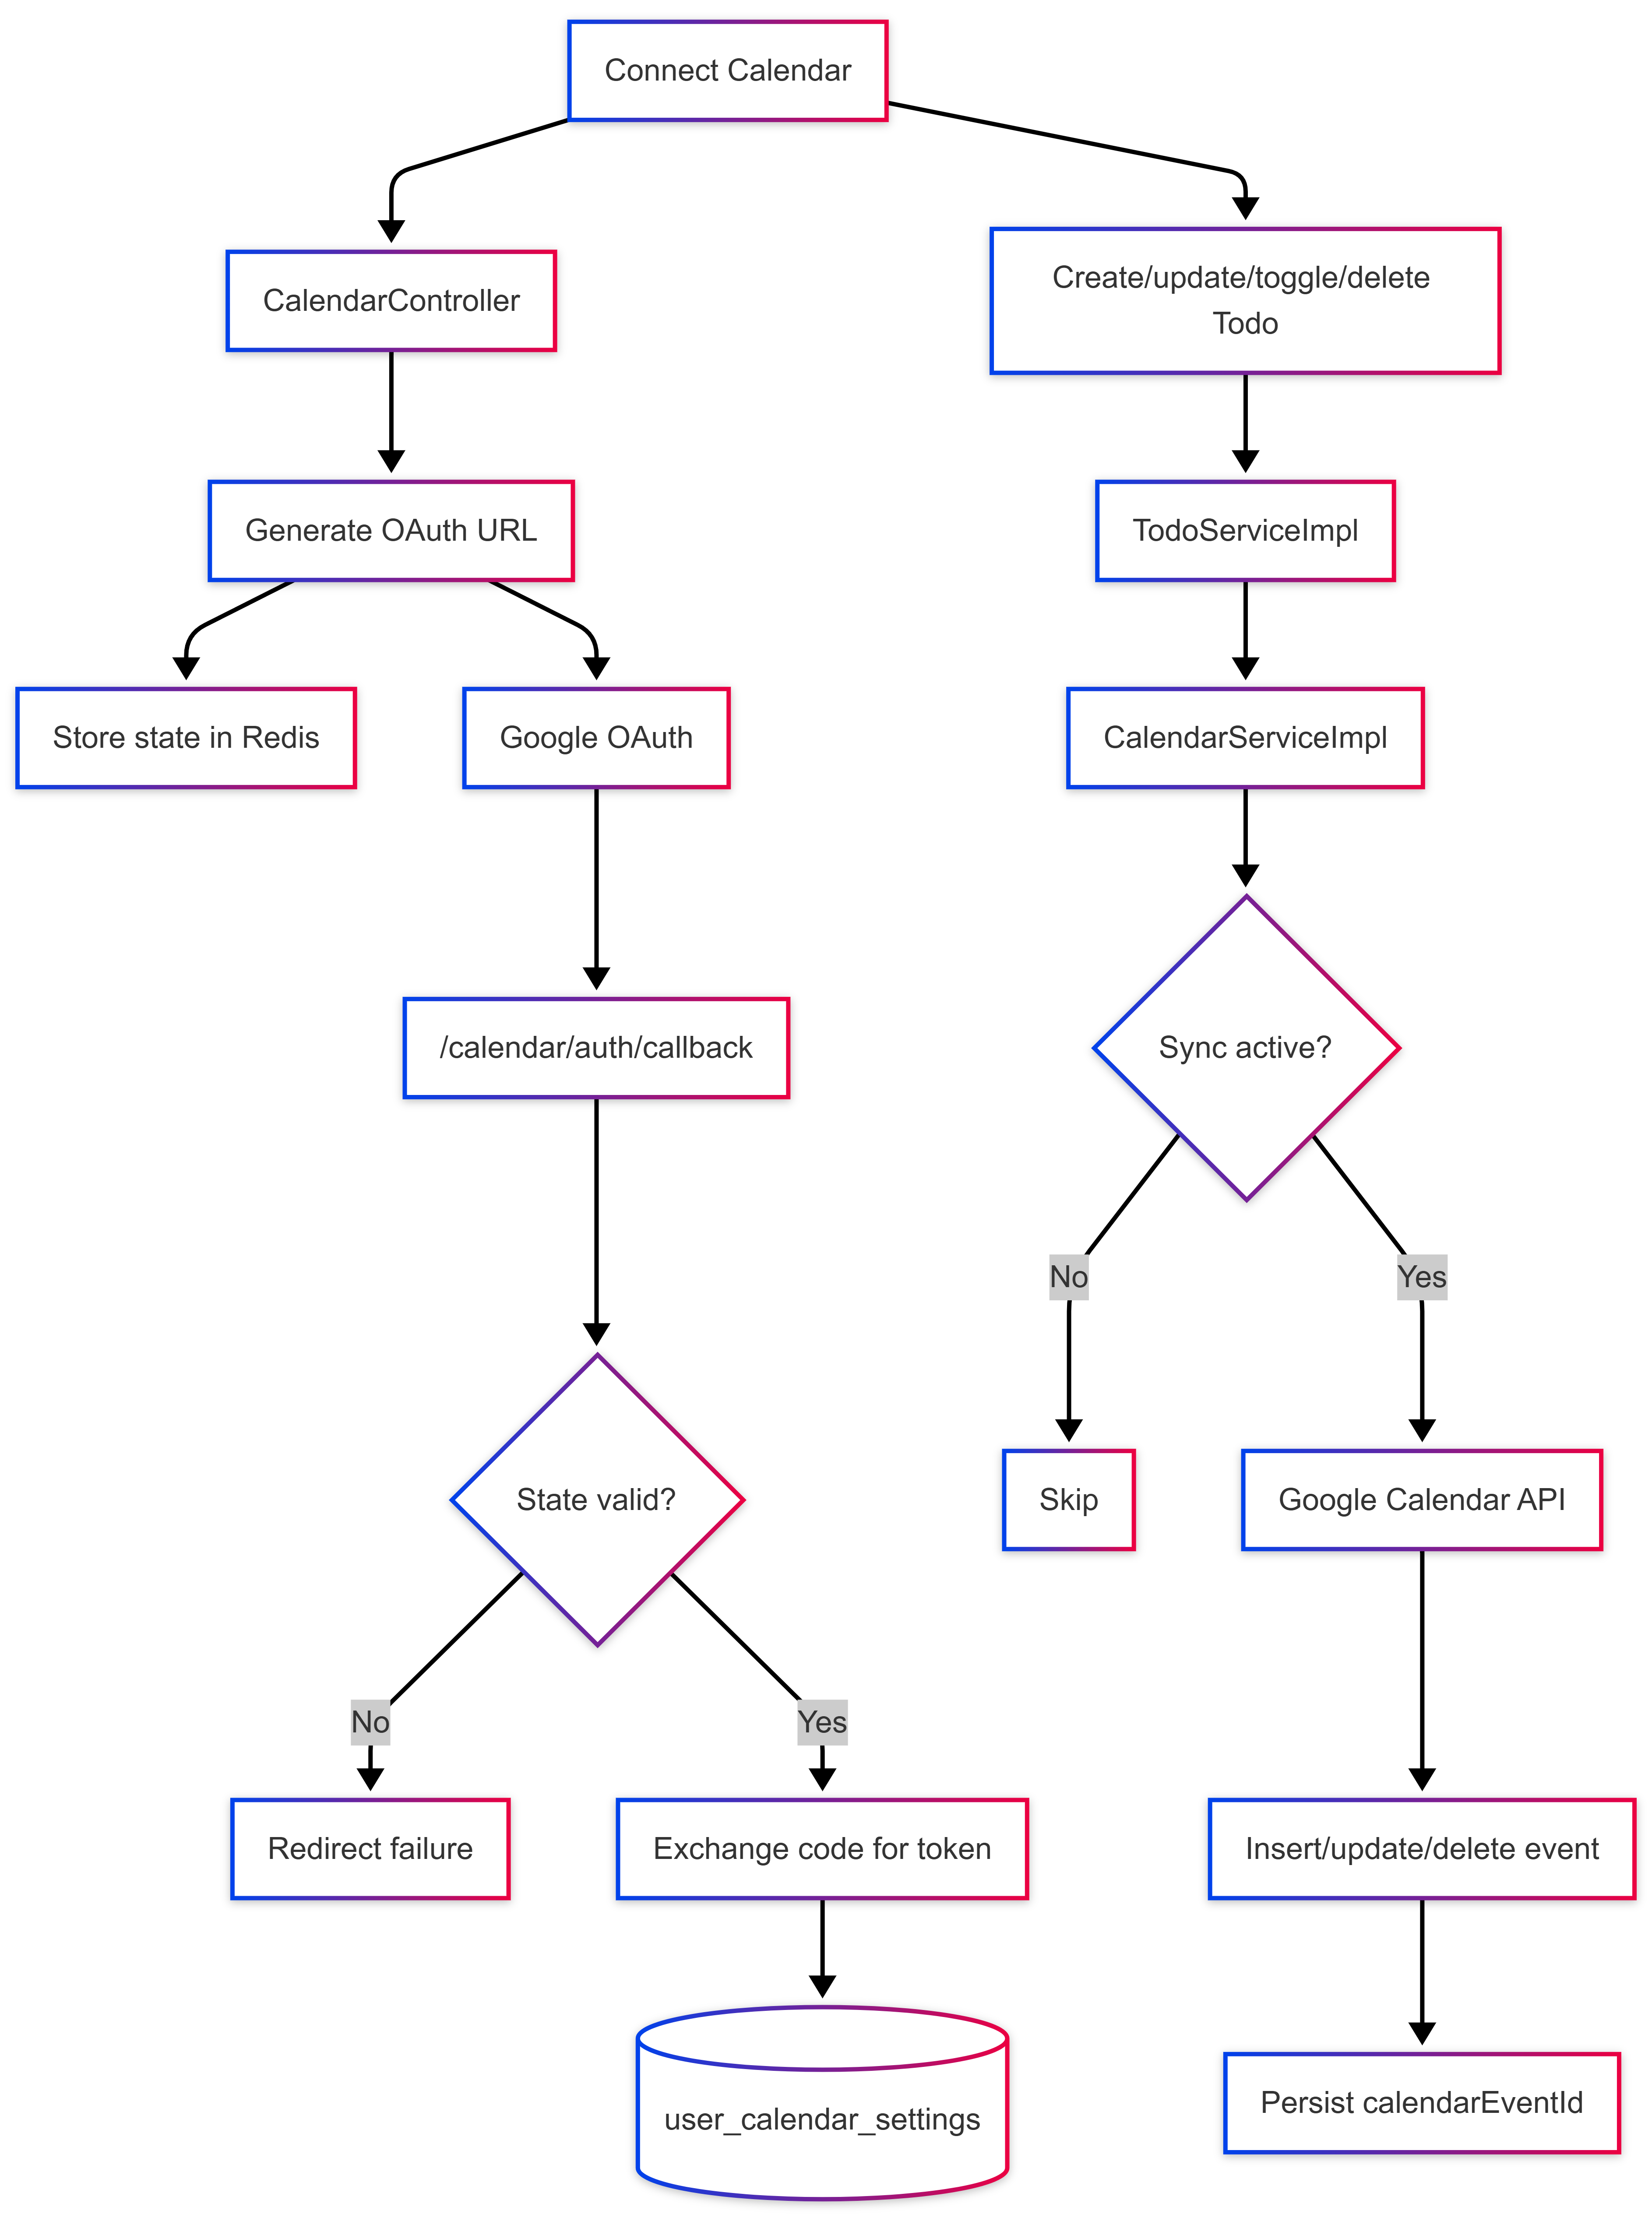
\includegraphics[width=1\textwidth,height=0.95\textheight,keepaspectratio]{images/chapter3/ProLearning_Arch-Detail_GgCalendar.drawio.png}
    \caption{Luồng đồng bộ Todo với Google Calendar}
    \label{fig:prolearning-architecture-detail_ggcalendar}
\end{figure}

\subsubsection{Thanh toán PayOS và kích hoạt tài khoản PRO}
\label{subsubsec:payos-pro-upgrade}

Luồng thanh toán được cài đặt theo hướng backend tạo payment link, lưu order ở trạng thái chờ và chỉ kích hoạt PRO sau khi nhận webhook hợp lệ từ PayOS. Webhook được xác minh chữ ký, đối chiếu order code và xử lý theo hướng idempotent để tránh cập nhật trùng hoặc payload giả mạo~\cite{payoswebhook}. Sau khi giao dịch thành công, backend lưu transaction, cập nhật subscription và phát sinh notification/email xác nhận.

\begin{figure}[htbp]
    \centering
    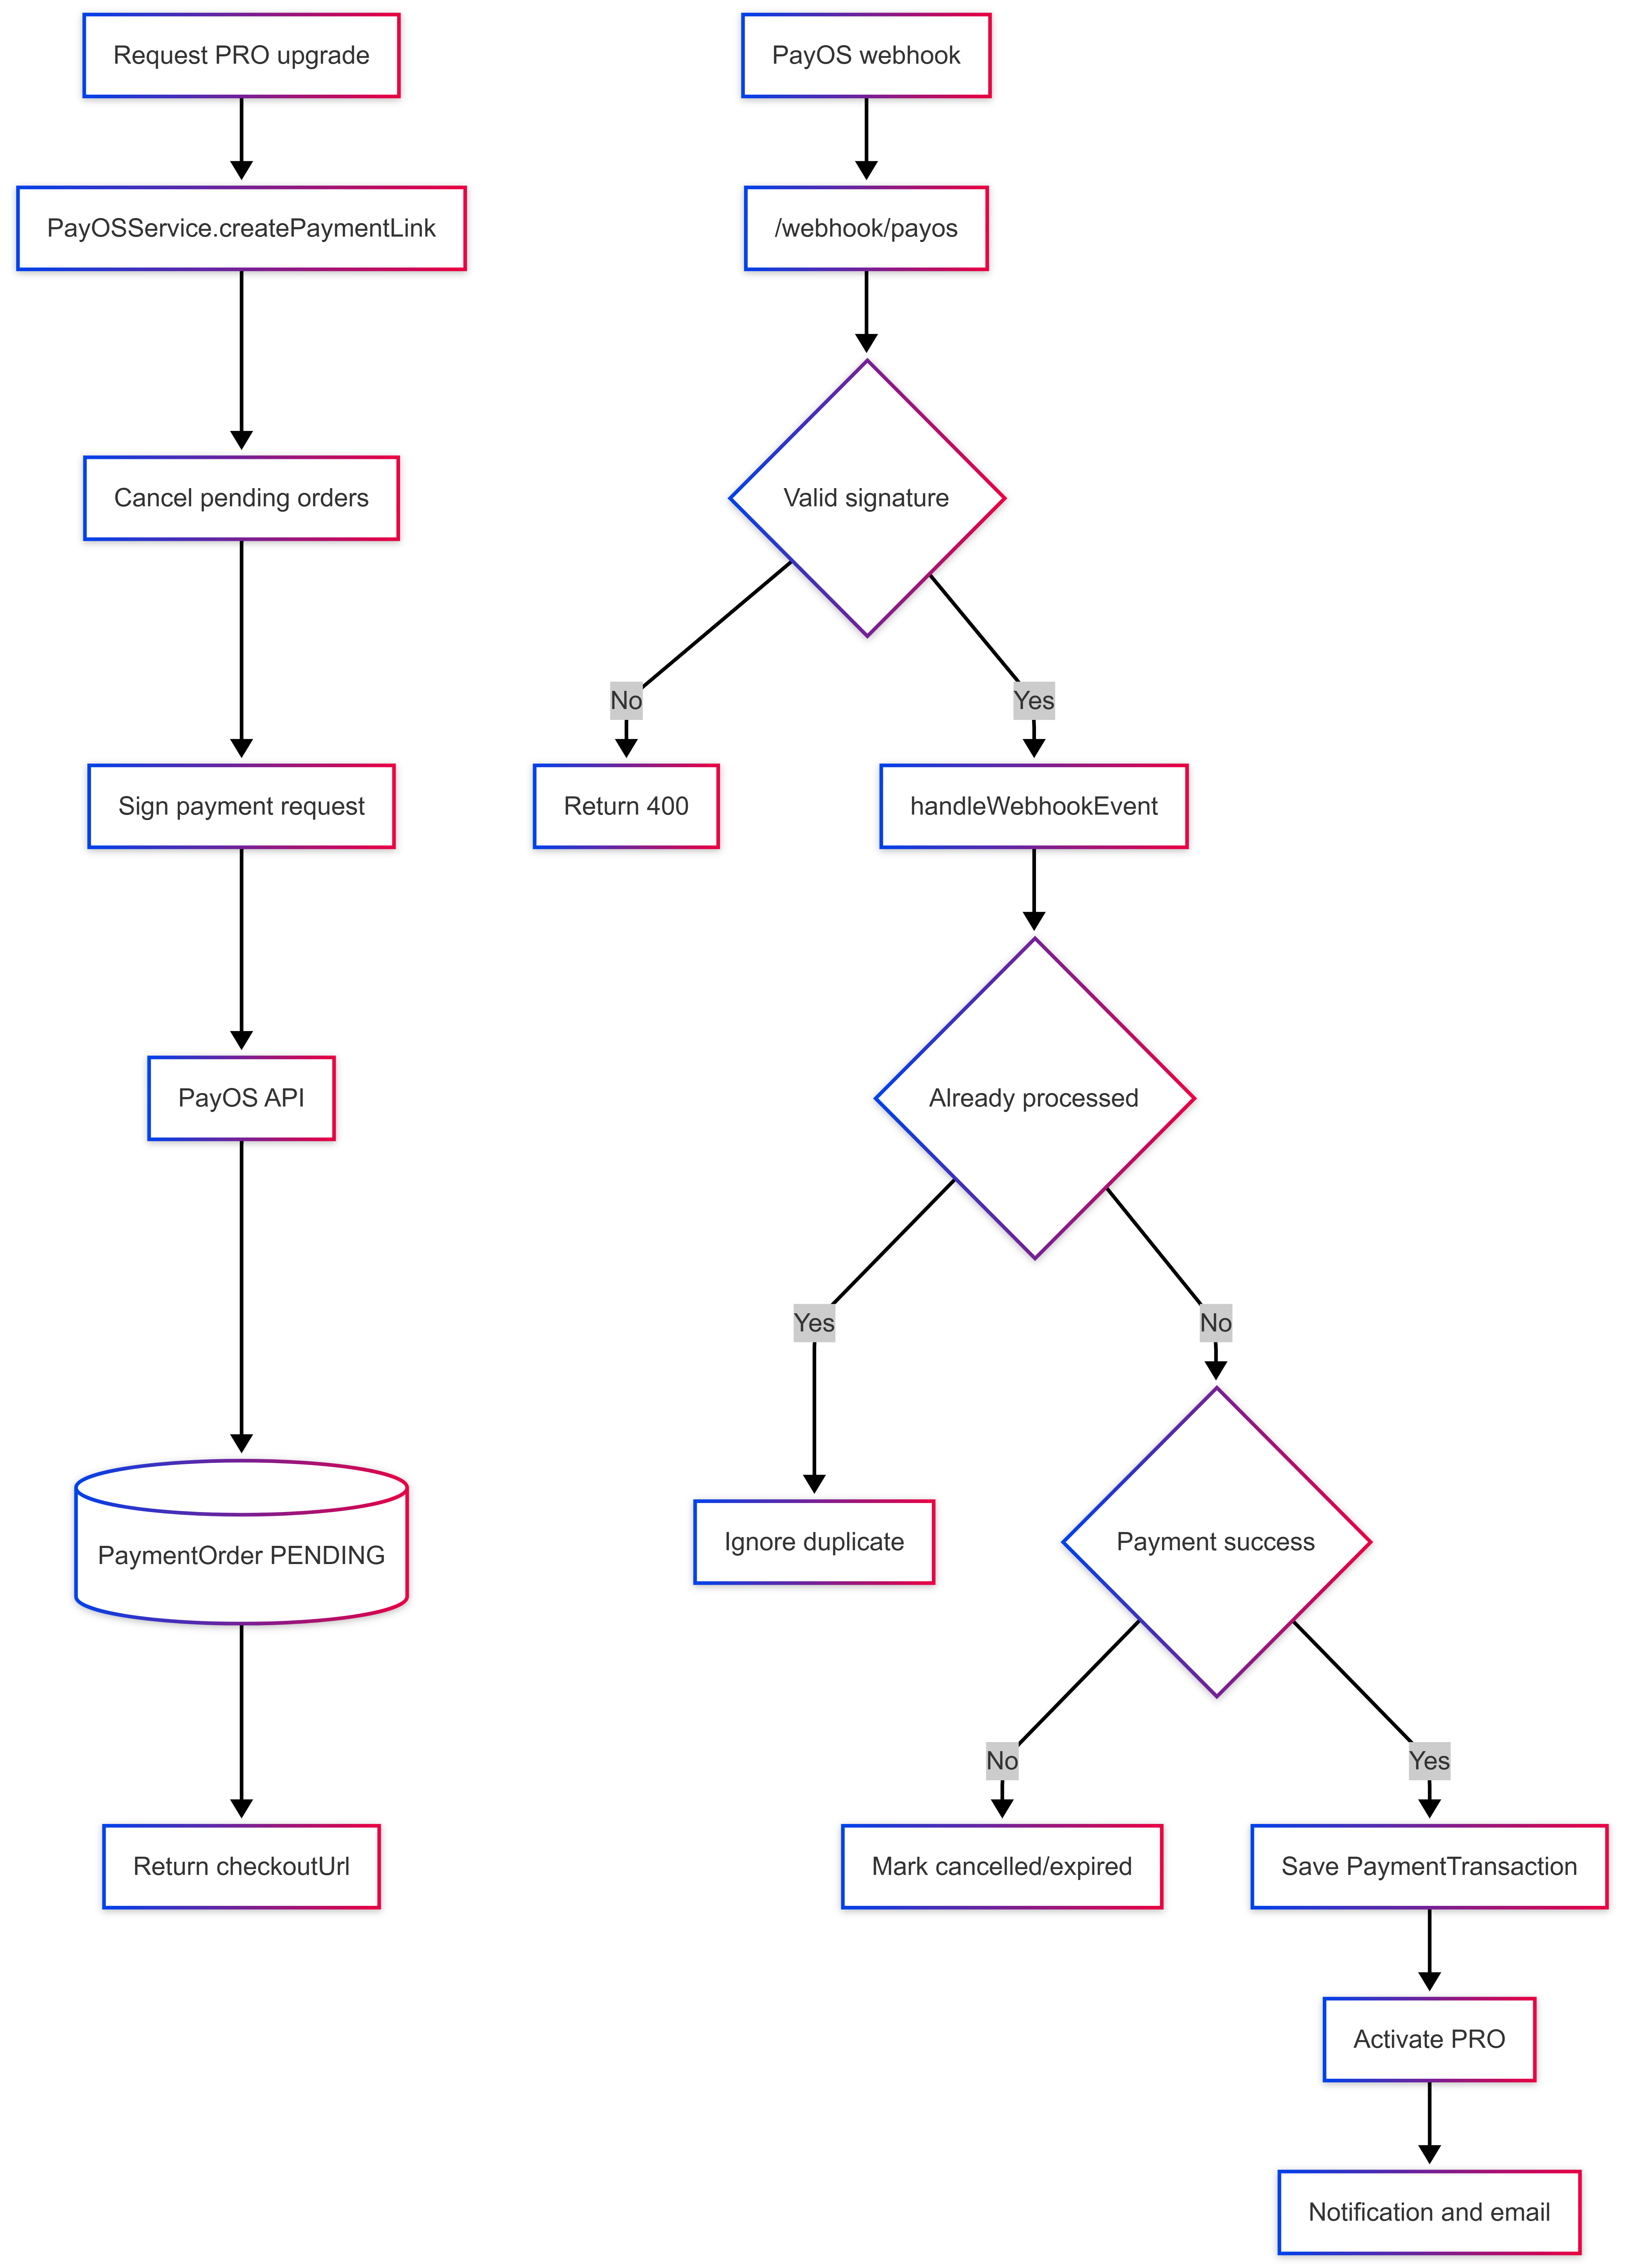
\includegraphics[width=1\textwidth,height=0.95\textheight,keepaspectratio]{images/chapter3/ProLearning_Arch-Detail_Payment_Gateway.drawio.png}
    \caption{Luồng thanh toán PayOS và nâng cấp tài khoản PRO}
    \label{fig:prolearning-architecture-detail_payment_gateway}
\end{figure}